\documentclass[]{article}

\usepackage{tikz}
\usepackage{amsmath}
\usepackage{amsfonts}
\usepackage{amssymb}
\usepackage{relsize}
\usepackage{tkz-base}
\usepackage{tkz-euclide}

\usetikzlibrary{svg.path}
\usetikzlibrary{arrows}
\usetikzlibrary{shapes.geometric,calc}

\newcommand{\crossout}[1]{\mathbin{\ooalign{${#1}$\cr\larger[1]{$\nearrow$}\cr}}}

%opening
\title{Inverse Kinematics I}
\author{Craig Carignan\\Glen Henshaw}

\begin{document}

\maketitle

\section{Overview}
Inverse kinematics is the problem of starting with a desired end effector pose $^{0}_{N}T$ and finding the joint angles $\underline{q}$ that cause the end effector to assume that pose. It is often the case that you will have not a single desired pose but a Cartesian curve or trajectory $^{0}_{N}T(t)$ and will want to find a trajectory in joint space $\underline{q}(t)$ that causes the end effector to follow the trajectory.

Note that while describing translational trajectories is pretty straightforward, using cubic splines or something equivalent, describing trajectories in rotation is a bit more complicated. It isn't that hard to use Euler of fixed angles, as long as you avoid the orientations where these descriptions become singular, but the fact that they do become singular at certain orientations means that 4--value descriptions such as quaternions is normally how it's done in practice. The math required to describe trajectories using quaternions is a bit beyond this course. For the following we'll assume that you have a single desired end effector pose.

\begin{figure}[h!]
	\centering
	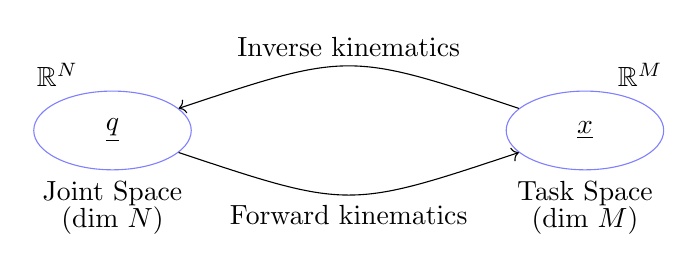
\begin{tikzpicture}
		\draw (0,0) node[shape=ellipse, draw=blue!50, minimum height=1cm, minimum width=2cm](angles){$\underline{q}$};
		\draw (-0.7,0.7) node{$\mathbb{R}^{N}$};
		\draw (0, -0.8) node{Joint Space};
		\draw (0, -1.15) node{(dim $N$)};
		\draw (6,0) node[shape=ellipse, draw=blue!50, minimum height=1cm, minimum width=2cm](cart){$\underline{x}$};
		\draw (6.7,0.7) node{$\mathbb{R}^{M}$};
		\draw (6, -0.8) node{Task Space};
		\draw (6, -1.15) node{(dim $M$)};
		\draw[->] (angles) .. controls (3, -1) .. (cart) node[pos=0.5][below] {Forward kinematics};
		\draw[->] (cart) .. controls (3, 1) .. (angles) node[pos=0.5][above] {Inverse kinematics};
	\end{tikzpicture}
\end{figure}

Formally, the problem is
\begin{eqnarray}
	\text{GIVEN:} & ^{0}_{N}T \nonumber\\
	\text{FIND:} & \underline{q} \nonumber
\end{eqnarray}
where
\begin{displaymath}
^{0}_{N}R, \ \!^{0}\underline{p}_{N} \Rightarrow \left\{\begin{array}{l} \text{6 independent equations}\\ \text{nonlinear}\\ \text{transcendental}\end{array}\right.
\end{displaymath}
\section{Workspace}
The \textit{workspace} is the Cartesian position and orientation subspace spanned by the manipulator, e.g. the set of all $\{x, y, z, \phi, \theta, \psi \}$ such that $\exists\  \underline{q}:\ \!^{B}_{T}T(\underline{q}) = \ \!^{B}_{T}T(x, y, z, \phi, \theta, \psi)$:
\begin{figure}[h!]
	\centering
	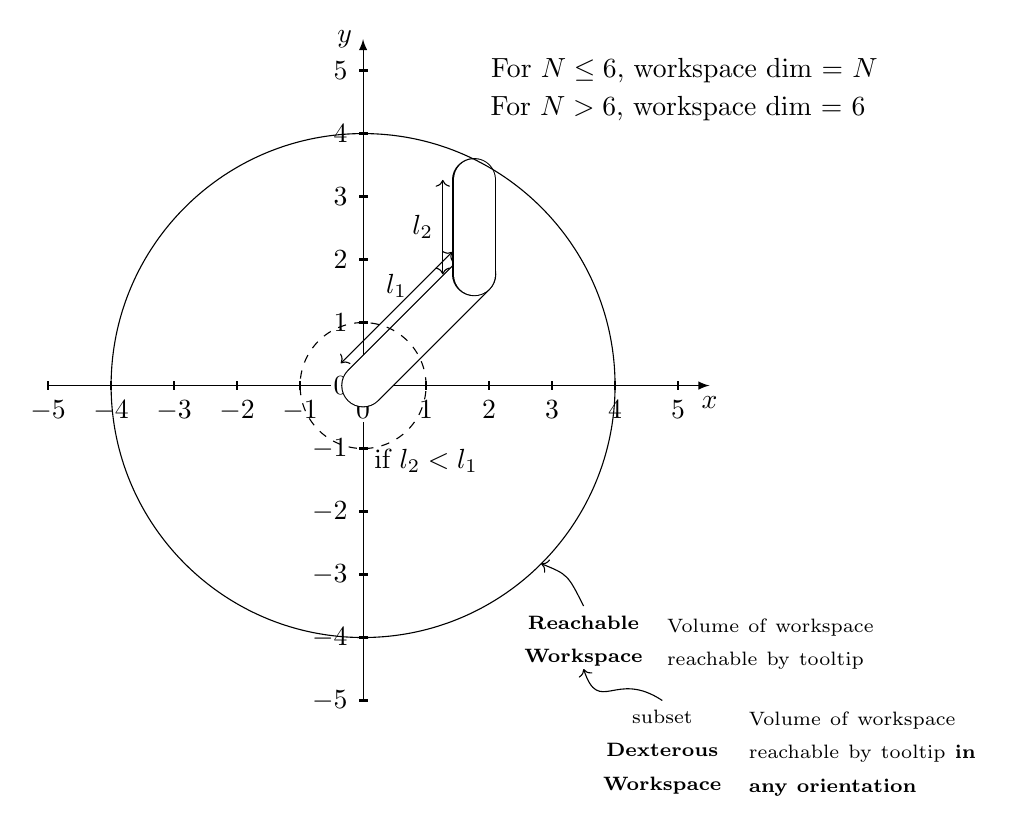
\begin{tikzpicture}[scale=0.8]
	\tkzInit[xmax=5,ymax=5,xmin=-5,ymin=-5]
	\tkzAxeXY
	
	\draw[cm={0.707,0.707,-0.707,0.707,(0,0)}][double=none, double distance=15pt, line join=round, line cap=round] (0.0, 0.0) -- (2.5, 0);
	\draw[cm={0.707,0.707,-0.707,0.707,(0,0)}][<->] (0, 0.5) -- (2.5, 0.5) node[above][pos=0.5]{$l_{1}$};	
	
	\draw[cm={0, 1, -1, 0,(1.765, 1.765)}][double=none, double distance=15pt, line join=round, line cap=round] (0.0, 0.0) -- (1.5, 0);
	\draw[cm={0, 1, -1, 0,(1.765, 1.765)}][<->] (0, 0.5) -- (1.5, 0.5) node[left][pos=0.5]{$l_{2}$};
	\draw (0,0) circle (4.0cm);
	\draw[dashed] (0,0) circle (1.0cm) node at (1,-1.2) {$\text{if } l_{2}<l_{1}$};
	
	\draw[->] (3.5, -3.5) node[text width=2cm,align=center,below]{\smaller[2]{\textbf{Reachable Workspace}}} .. controls (3.25, -3) .. (0.707*4, 0.707*-4);
	\draw (6.7, -4.1) node[text width=3cm]{\smaller[2]{Volume of workspace reachable by tooltip}};
	\draw[->] (4.75, -5) node[text width=2cm,align=center,below]{\smaller[2]{subset \textbf{Dexterous Workspace}}} .. controls (4, -4.5) and (3.75, -5.25) .. (3.5, -4.5);
	\draw (8, -5.85) node[text width=3cm]{\smaller[2]{Volume of workspace reachable by tooltip \textbf{in any orientation}}};

	\draw (5.1,5) node{For $N \le 6$, workspace dim = $N$};
	\draw (5,4.4) node{For $N>6$, workspace dim = 6};
	\end{tikzpicture}
\end{figure}

\section{Closed--form Solutions}
In some case you can find a closed--form solution for the inverse kinematics of a manipulator.


\subsection{Example: 3--link planar manipulator}
\begin{figure}
	\centering
	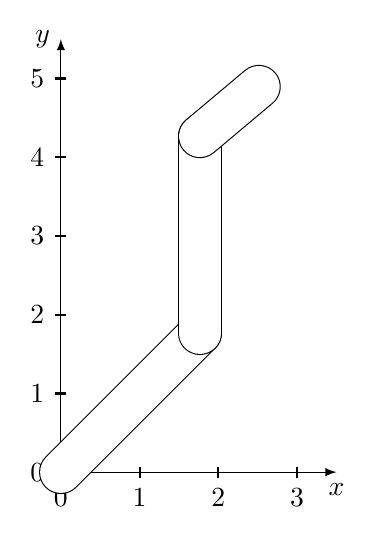
\begin{tikzpicture}
	\tkzInit[xmax=3,ymax=5,xmin=0,ymin=0]
	\tkzAxeXY
	\draw[cm={0.707,0.707,-0.707,0.707,(0,0)}][double=none, double distance=15pt, line join=round, line cap=round] (0.0, 0.0) -- (2.5, 0);
		
	\draw[cm={0, 1, -1, 0,(1.765, 1.765)}][double=none, double distance=15pt, line join=round, line cap=round] (0.0, 0.0) -- (2.5, 0);
	
	\draw[cm={0.75,0.63,-0.63,0.75,(1.765, 1.765+2.5)}][double=none, double distance=15pt, line join=round, line cap=round] (0.0, 0.0) -- (1, 0);
	
	\end{tikzpicture}
	\caption{Three--link planar manipulator}
\end{figure}

For this particular manipulator we can find a close--form solution for $\theta_{1}, \theta_{2}, \theta_{3}$. In fact there are two ways to go about it, an algebraic approach and a geometric approach. You can see the details of the geometric approach in section 4.4 of the textbook. I'll do the algebraic one here.

Set $^{0}_{3}T = \ \!^{0}_{W}T_{goal}$...

\begin{displaymath}
^{0}_{3}T = \left[ \begin{array}{ccc|c} c_{123} & -s_{123} & 0 & l_{1}c_{1}+l_{2}c_{12} \\ s_{123} & c_{123} & 0 & l_{1}s_{1} + l_{2}s_{12} \\ 0 & 0 & 1 & 0 \\ \hline 0 & 0 & 0 & 1
\end{array}\right]
\end{displaymath}
and
\begin{displaymath}
^{B}_{W}T = \left[ \begin{array}{ccc|c} c_{\phi} & -s_{\phi} & 0 & x \\ s_{\phi} & c_{\phi} & 0 & y \\ 0 & 0 & 1 & 0 \\ \hline 0 & 0 & 0 & 1
\end{array}\right]
\end{displaymath}
So we can, by inspection, get four equations that have to be solved for $\theta_{1}, \theta_{2}, \theta_{3}$:
\begin{eqnarray}
c_{\phi} & = & c_{123} \label{linearc} \\
s_{\phi} & = & s_{123} \label{linears} \\
x & = & l_{1}c_{1}+l_{2}c_{12} \label{linearx} \\
y & = & l_{1}s_{1} + l_{2}s_{12} \label{lineary}
\end{eqnarray}
We can square \ref{linearx} and \ref{lineary} and add them:
\begin{displaymath}
x^{2}+y^{2} = l_{1}^{2} + l_{2}^{2} + 2l_{1}l_{2}c_{2}
\end{displaymath}
and solve for $c_{2}$:
\begin{displaymath}
c_{2}=\frac{x^{2}+y^{2}-l_{1}^{2}-l_{2}^{2}}{2l_{1}l_{2}}
\end{displaymath}
You can then get $s_{2} = \pm \sqrt{1-c_{2}^{2}}$ and then $\theta_{2} = \text{atan2}(s_{2}, c_{2})$.

We can then solve for $\theta_{1}$. This is a bit involved, but it's a pattern that occurs a lot in inverse kinematics.

First, substitute $k_{1} = l_{1} + l_{2}c_{2}$ and $k_{2} = l_{2}s_{2}$ into Eqs. \ref{linearc} and \ref{linears}. This makes the structure of the equations a bit clearer:
\begin{eqnarray}
x & = & k_{1}c_{1} - k_{2}s_{1} \label{cleanx} \\ y & = & k_{1}s_{1} + k_{2}c_{1} \label{cleany}
\end{eqnarray}
Now we can use a change of variables. Specifically, we're going to change from Cartesian to polar coordinates, as shown in the diagram:
\begin{figure}[h!]
	\centering
	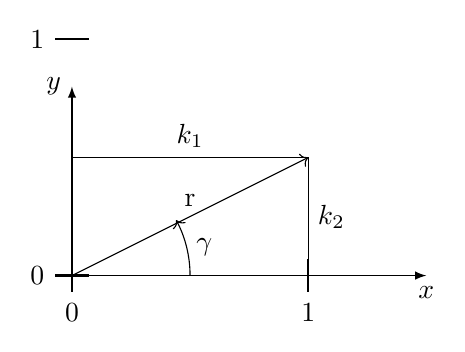
\begin{tikzpicture}[scale=3]
 		\tkzInit[xmax=1,ymax=0.3,xmin=0,ymin=0]
		%\tkzGrid
		\tkzAxeXY

		\draw[->] (0,0) -- (1, 0.5) node[pos=0.5, above] {r};
		\draw[->] (0.5, 0) arc(0:28:0.5cm) node[right][pos=0.5]{$\gamma$};
		\draw (1, 0) -- (1, 0.5) node[pos=0.5, right] {$k_{2}$};
		\draw (0, 0.5) -- (1, 0.5) node[pos=0.5, above] {$k_{1}$};
	\end{tikzpicture}
\end{figure}

Define $r = \sqrt{k_{1}^{2} + k_{2}^{2}}$ and $\gamma = \text{atan2}(k_{2}, k_{1})$. Then
\begin{eqnarray}
	k_{1} & = & r \cos{\gamma} \\
	k_{2} & = & r \sin{\gamma}
\end{eqnarray}
	
We can now write Eqs. \ref{cleanx} and \ref{cleany} as
\begin{eqnarray}
\frac{x}{r} & = & \cos{\gamma}\cos{\theta_{1}} - \sin{\gamma}\sin{\theta_{1}} \nonumber\\
\frac{y}{r} & = & \cos{\gamma}\sin{\theta_{1}} + \sin{\gamma}\cos{\theta_{1}} \nonumber
\end{eqnarray}
or
\begin{eqnarray}
	\cos{\gamma+\theta_{1}} & = & \frac{x}{r} \\
	\sin{\gamma+\theta_{1}} & = & \frac{y}{r}
\end{eqnarray}
We can then find
\begin{displaymath}
\gamma+\theta_{1} = \text{atan2}(\frac{y}{r},\frac{x}{r}) = \text{atan2}(y,x)
\end{displaymath}
Therefore
\begin{displaymath}
\theta_{1} = \text{atan2}(y,x) - \text{atan2}(k_{2},k_{1})
\end{displaymath}
And then using Eqs. \ref{linearc} and \ref{linears} you can solve for $\theta_{3}$:
\begin{equation}
\theta_{1}+\theta_{2}+\theta_{3} = \text{atan2}(s_{\phi}, c_{\phi}) = \phi \rightarrow \theta_{3} = \phi - \theta_{1} - \theta_{2}
\end{equation}
 
Note that there are in fact two solutions to the inverse kinematics problem in this case, as illustrated in the diagram below:
 
\begin{figure}[h!]
 	\centering
 	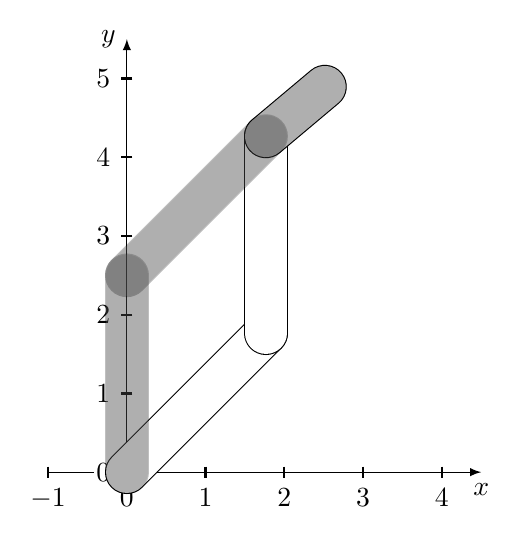
\begin{tikzpicture}
 	\tkzInit[xmax=4,ymax=5,xmin=-1,ymin=0]
 	%\tkzGrid
 	\tkzAxeXY

	\draw[cm={0.707,0.707,-0.707,0.707,(0,0)}][double=none, double distance=15pt, line join=round, line cap=round] (0.0, 0.0) -- (2.5, 0);

	\draw[cm={0, 1, -1, 0,(1.765, 1.765)}][double=none, double distance=15pt, line join=round, line cap=round] (0.0, 0.0) -- (2.5, 0);

	\draw[cm={0.75,0.63,-0.63,0.75,(1.765, 1.765+2.5)}][double=none, double distance=15pt, line join=round, line cap=round] (0.0, 0.0) -- (1, 0);

 	\draw[cm={0,1,-1,0,(0,0)}][double=gray, double distance=15pt, line join=round, line cap=round, draw opacity = 0.25] (0.0, 0.0) -- (2.5, 0);

	\draw[cm={0.707,0.707,-0.707,0.707,(0, 2.5)}][double=gray, double distance=15pt, line join=round, line cap=round, draw opacity = 0.25] (0.0, 0.0) -- (2.5, 0);

	\draw[cm={0.75,0.63,-0.63,0.75,(1.765, 1.765+2.5)}][double=gray, double distance=15pt, line join=round, line cap=round, draw opacity = 0.25] (0.0, 0.0) -- (1, 0);
 	\end{tikzpicture}
 \end{figure}

And you can also see this by virtue of the fact that in the derivation above we chose $s_{2} = \pm \sqrt{1-c_{2}^{2}}$. You get to choose the sign --- one choice corresponds to the elbow--up configuration and the other to the elbow--down configuration.

Closed--form solutions are great when you can find them. They are numerically stable (they always return exactly the same result, to the limit of the precision of the computer you are using) and can be calculated quickly. Unfortunately, in general there is no straightforward way to find a closed--form expression for the kinematics of a given robotic manipulator. There isn't even a guarantee that a closed--form solution exists.

 
\subsection{Pieper's Method}
 There is, however, one important case in which a closed--form solution can be found: when \begin{itemize} \item you have a 6 DOF arm; and \item three consecutive axes intersect at a point (usually the first three or the last three).\end{itemize}
 This requirement means that the problem can be decomposed into two successive 3--DOF problems. By far the most common case is a revolute manipulator where the last three rotational axes intersect; this is sometimes known as a \textit{spherical wrist}. It implies that the point of intersection is at the origin of all three frames.
 
 This technique is called ``Pieper's Method''.
 
 The key observation is that $^{0}\underline{p}_{4} = \ \!^{0}\underline{p}_{5} = \ \!^{0}\underline{p}_{6}$.
 
 Steps:
 
 \begin{itemize}
 	\item Solve for $^{0}\underline{p}_{4}$:
 	\begin{displaymath} ^{0}\underline{p}_{T} = \ \!^{0}\underline{p}_{4} + \ \!^{0}_{4}R\ \!\crossout{^{4}\underline{p}_{6}}^{0} + \underbrace{^{0}_{6}R}_{=\ \!^{0}_{T}R}\underbrace{\ \!^{6}\underline{p}_{T}}_{\text{\ given}} \end{displaymath}
 	\item Solve for $\theta_{1}$, $\theta_{2}$, and $\theta_{3}$:
 	\begin{displaymath} ^{0}\underline{p}_{4} = \ \!^{0}_{1}T(\theta_{1})\ \!^{1}_{2}T(\theta_{2})\ \!^{2}_{3}T(\theta_{3})\underbrace{^{3}\underline{p}_{4}}_{\text{given}} \end{displaymath}
 	Note that this gives three equations in three unknowns.
 	\item Solve for $\theta_{4}$, $\theta_{5}$, and $\theta_{6}$:
 	\begin{displaymath}
 	^{0}_{T}R = \underbrace{^{0}_{3}R}_{\substack{\text{for}\\\theta_{1}-\theta_{3}}}\underbrace{^{3}_{6}R}_{\substack{\text{for}\\\theta_{4}-\theta_{6}}}\underbrace{^{6}_{T}R}_{=I}
 	\end{displaymath}
 	\begin{displaymath}
 		^{3}_{6}R = \ \!^{0}_{3}R(\theta_{1}, \theta_{2}, \theta_{3})^{T}\ \!^{0}_{T}R
 	\end{displaymath}
 	Note that this also gives three equations in three unknowns.
 \end{itemize}
 
\end{document}
